\chapter{Presentaci\'on y an\'alisis de resultados}
\section{Distancias de profundidades recomendadas entre el atleta y el sensor} \label{res:idMov}
En la siguiente tabla se muestra un resumen general de las caracter\'isticas de la muestra de cada equipo deportivo, en ella se describe la altura promedio y las distancias recomendadas para ejecutar correctamente el seguimiento del esqueleto (renderizaci\'on completa del esqueleto humano), dichos datos fueron capturados por el sensor Kinect a una altura de 0.70 metros desde el suelo y tomando como punto de referencia, la cadera central de cada atleta:
\begin{table}[H]
\begin{center}
\caption{Distancias de profundidades recomendadas para el funcionamiento del seguimiento del  esqueleto}
\label{tab:depthCalculation}
\begin{tabular}{lllll}
\hline
\multicolumn{3}{|c|}{Caracter\'isticas generales} & \multicolumn{2}{l|}{\begin{tabular}[c]{@{}l@{}}Distancias de profundidades recomendadas \\ entre el usuario y el sensor\end{tabular}} \\ \hline
\multicolumn{1}{|l|}{Deporte} & \multicolumn{1}{l|}{\begin{tabular}[c]{@{}l@{}}Altura promedio\\ (metros)\end{tabular}} & \multicolumn{1}{l|}{\begin{tabular}[c]{@{}l@{}}Desviaci\'on est\'andar\\ de la altura (metros)\end{tabular}} & \multicolumn{1}{l|}{\begin{tabular}[c]{@{}l@{}}M\'inima\\ (metros)\end{tabular}} & \multicolumn{1}{l|}{\begin{tabular}[c]{@{}l@{}}M\'axima\\ (metros)\end{tabular}} \\ \hline
\multicolumn{1}{|l|}{Tenis de mesa} & \multicolumn{1}{l|}{1.302435} & \multicolumn{1}{l|}{+/- 0.088683} & \multicolumn{1}{l|}{3.505103} & \multicolumn{1}{l|}{3.990376} \\ \hline
\multicolumn{1}{|l|}{Animaci\'on} & \multicolumn{1}{l|}{1.342471} & \multicolumn{1}{l|}{+/-0.059301} & \multicolumn{1}{l|}{2.763813} & \multicolumn{1}{l|}{3.411942} \\ \hline
\multicolumn{1}{|l|}{Taekwondo} & \multicolumn{1}{l|}{1.373372} & \multicolumn{1}{l|}{+/-0.098490} & \multicolumn{1}{l|}{2.556640} & \multicolumn{1}{l|}{3.869427} \\ \hline
\multicolumn{5}{l}{\textbf{Fuente:} Datos capturados por los atletas}
\end{tabular}
\end{center}
\end{table}
\section{Muestras de fotogramas del movimiento} \label{res:fotogramas}
En esta secci\'on se realiz\'o por cada equipo deportivo, una tabla en donde se muestra las  fotogramas del seguimiento del  esqueleto de cada atleta (utilizados para los entrenamientos y los testeos del algoritmo Random Forest Regression), con la finalidad de mostrar distintas formas correctas para ejecutar un paso (de acuerdo al profesional). As\'i mismo por cada fotograf\'ia se muestra cuatros elementos importantes:
\begin{itemize}
\item El fondo de color negro.
\item El piso representado por cuadros de colores grises.
\item La figura del atleta figurado por una sombra de color gris.
\item El seguimiento del esqueleto conformado por puntos (articulaciones) y l\'ineas de color blanco (uni\'on de dos articulaciones).
\end{itemize}
\begin{figure}[H]
	\caption{Fotogramas de 6 sujetos del equipo de tenis de mesa}
	\label{fig:fotogramaTenis}
	\centering
	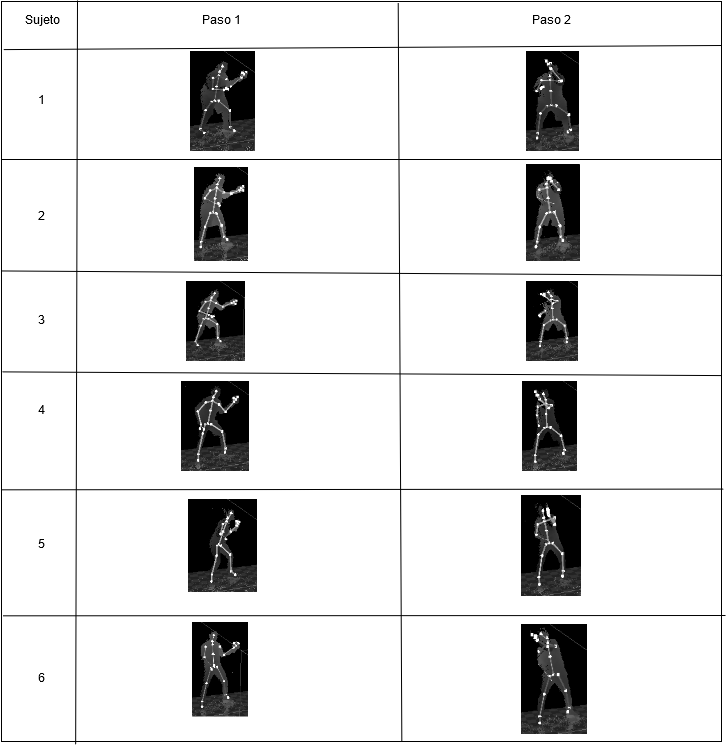
\includegraphics[width=445px,height=560px]{graphics/resultados/SETenisDeMesa.PNG} \\
	\textbf{Fuente:} Recuperado por los v\'ideos de trabajo de campo (ver instrumento \ref{ins:KinectStudio})
\end{figure}
\begin{figure}[H]
	\caption{Fotogramas de 7 sujetos del equipo de animaci\'on}
	\label{fig:fotogramaCheerleader}
	\centering
	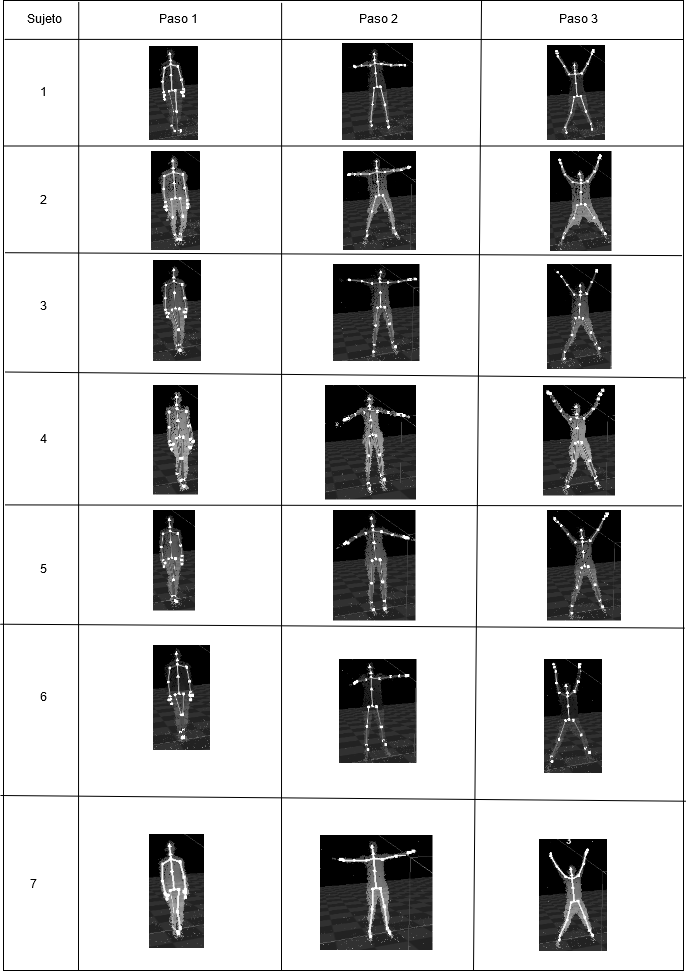
\includegraphics[width=445px,height=600px]{graphics/resultados/SECheerleaders.PNG} \\
	\textbf{Fuente:} Recuperado por los v\'ideos de trabajo de campo (ver instrumento \ref{ins:KinectStudio})
\end{figure}
\begin{figure}[H]
	\caption{Fotogramas de 7 sujetos del equipo de taekwondo}
	\label{fig:fotogramaTaekwondo}
	\centering
	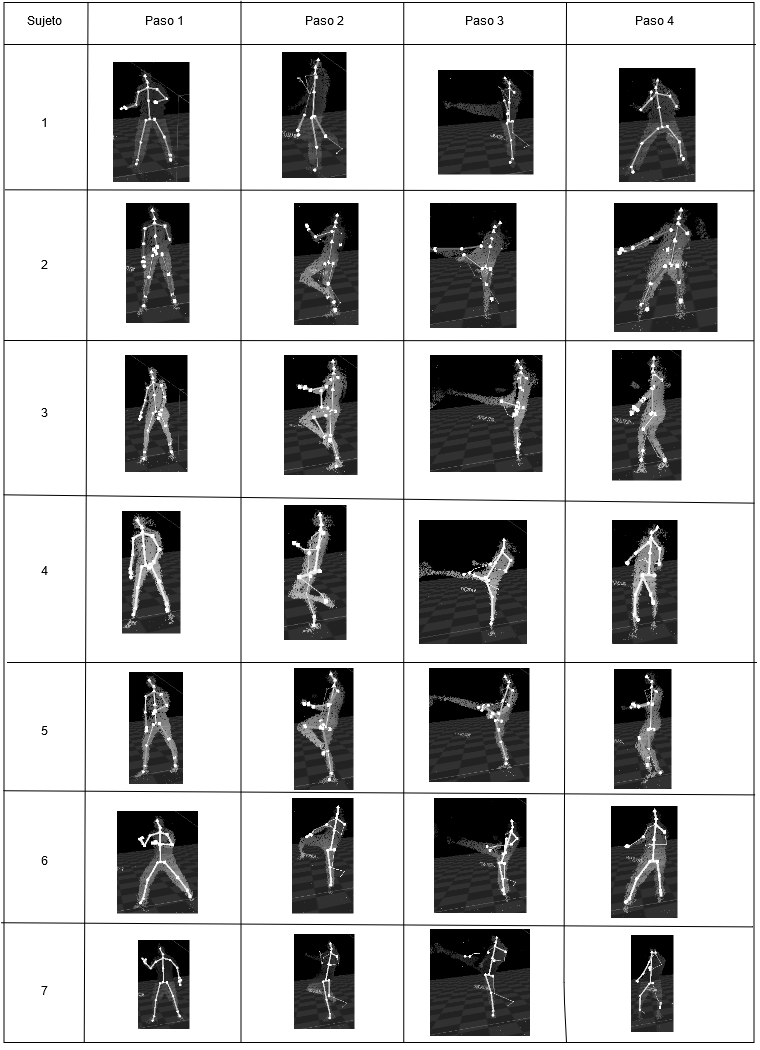
\includegraphics[width=445px,height=600px]{graphics/resultados/SETaekwondo.PNG} \\
	\textbf{Fuente:} Recuperado por los v\'ideos de trabajo de campo (ver instrumento \ref{ins:KinectStudio})
\end{figure}
\begin{landscape}
\section{Razones de fallo del seguimiento del esqueleto}
El seguimiento del esqueleto es un elemento  fundamental en cada fotograma, sin embargo se debe tomar en cuenta que puede fallar por varias razones, entre ellas se encuentran las siguientes fallas: del atleta (hombre), del sensor Kinect (m\'aquina), del lugar de trabajo (entorno y  medida), de la interacci\'on  con objetos o elementos externos (material) y de la preparaci\'on necesaria para realizar una rutina (m\'etodo):
\begin{figure}[H]
	\caption{Diagrama de ishikawa sobre el fallo del seguimiento del esqueleto}
	\label{fig:ishikawa}
	 \begin{center}
	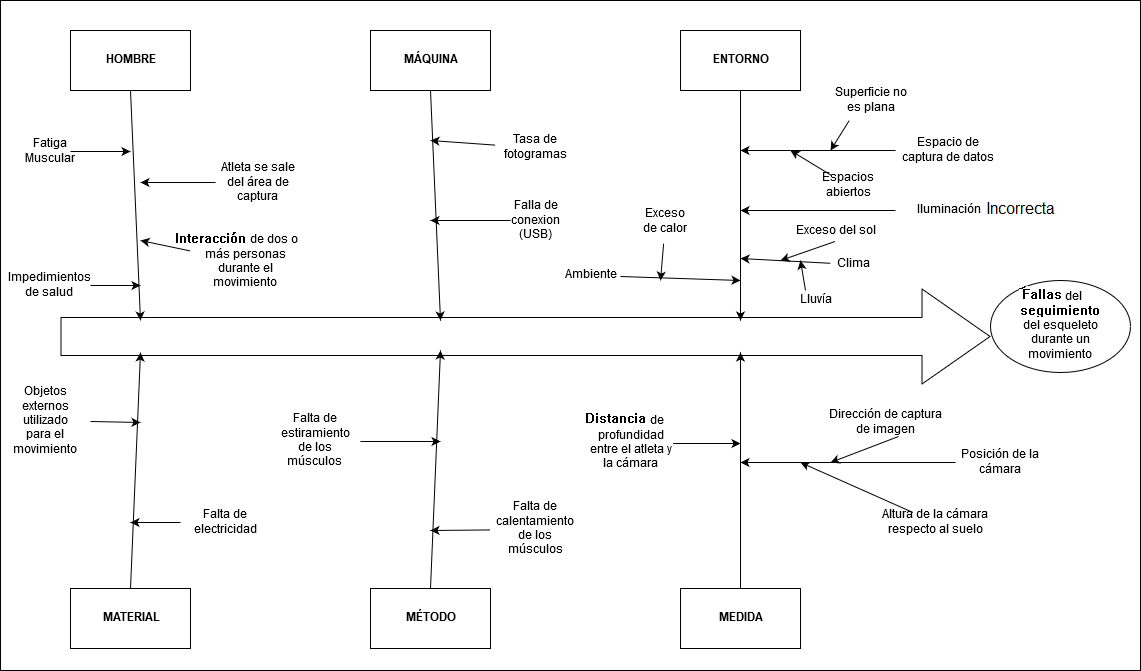
\includegraphics[width=500px,height=270px]{graphics/resultados/Ishi-SeguimientoDeEsqueleto.PNG}	 \\
	\end{center}
	\textbf{Fuente:} Este diagrama fue realizado con base a las observaciones del trabajo de campo, la cual el investigador observ\'o los sucesos en que fallaban el seguimiento del esqueleto, como por ejemplo las interrupciones de personas (generaba dos o m\'as seguimientos de esqueletos) u objetos externos (interrupciones de pelotas de otros deportes), las fallas del hardware o software (falta de alimentaci\'on de energ\'ia), fallas en el ambiente que fue instalado el prototipo (exceso de calor, espacios cerrados, lluv\'ia, la iluminaci\'on incorrecta), fallas de la medici\'on (posici\'on del atleta o el sensor) y  fallas con respecto a la preparaci\'on del atleta (falta de calentamiento o impedimentos del salud del atleta, que conllevaba a realizar repeticiones no v\'alidas).
\end{figure}
\end{landscape}
\section{Proceso de etiquetaci\'on de un movimiento}
Consta de un conjunto de paneles de etiquetaciones de fotogramas, que se utilizaron para los entrenamientos y los testeos del algoritmo Random Forest Regression (reconocimiento de los pasos de un movimiento v\'alido), adem\'as por cada panel se debe tomar en cuenta los  siguientes elementos:
\begin{itemize}
\item Una l\'inea curvada (con forma de ese "S") que unifica 2 o m\'as puntos (representaci\'on de una repetici\'on que pasa por cada paso de un  movimiento v\'alido).
\item Espacios de color gris (momentos en que no se est\'a realizando un movimiento v\'alido).
\end{itemize}
As\'i mismo, estos resultados demuestran dos caracter\'isticas de la muestra de cada equipo deportivo:
\begin{itemize}
\item  La cantidad total de repeticiones de movimientos por atleta.
\item Cada atleta tiene distintas habilidades f\'isicas, debido que algunos realizaron m\'as repeticiones de lo solicitado (atletas que llevaban un tiempo en el equipo deportivo) y otros no (nuevos atletas del equipo deportivo).
\end{itemize}
\begin{table}[H]
	\caption{Etiquetaci\'on de fotogramas del equipo de tenis de mesa}
	\label{fig:etiquetaTenis}
	\centering
	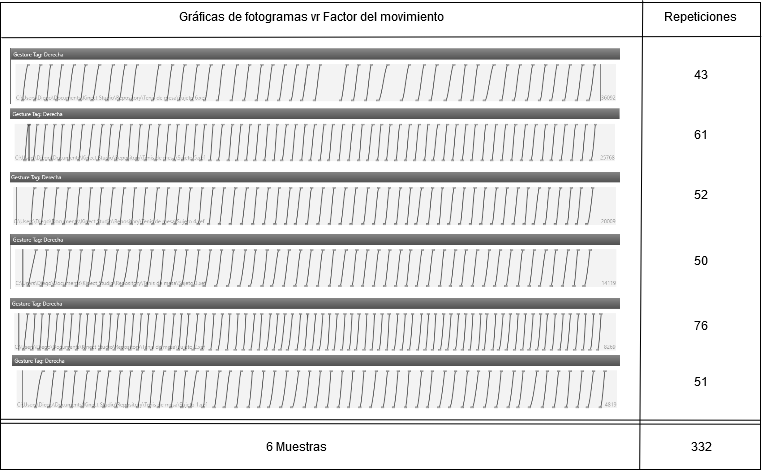
\includegraphics[width=445px,height=260px]{graphics/resultados/GraSegTenisDeMesa.PNG} \\
	\textbf{Fuente:} Recuperado por los v\'ideos etiquetados del trabajo de campo (ver instrumento \ref{ins:VisualGestureBuilder})
\end{table}
\begin{table}[H]
	\caption{Etiquetaci\'on de fotogramas del equipo de animaci\'on}
	\label{fig:etiquetaCheerleader}
	\centering
	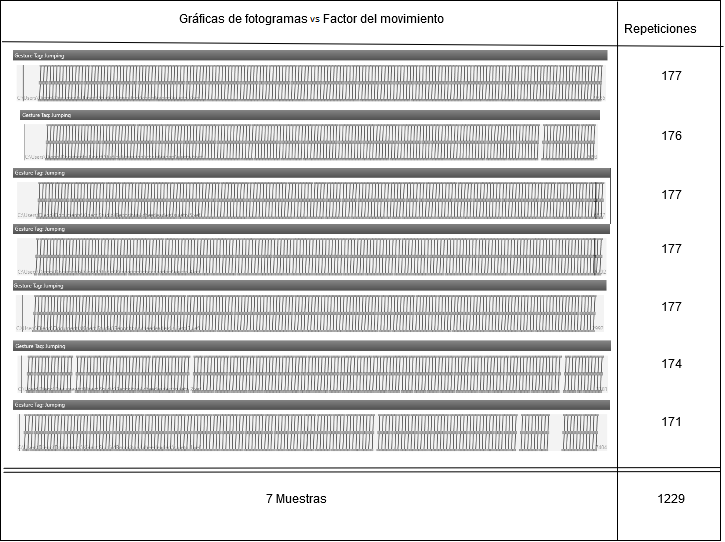
\includegraphics[width=445px,height=220px]{graphics/resultados/GraSegCheerleaders.PNG} \\
	\textbf{Fuente:} Recuperado por los v\'ideos etiquetados del trabajo de campo (ver instrumento \ref{ins:VisualGestureBuilder})
\end{table}
\begin{table}[H]
	\caption{Etiquetaci\'on de fotogramas del equipo de taekwondo}
	\label{fig:etiquetaTaekwondo}
	\centering
	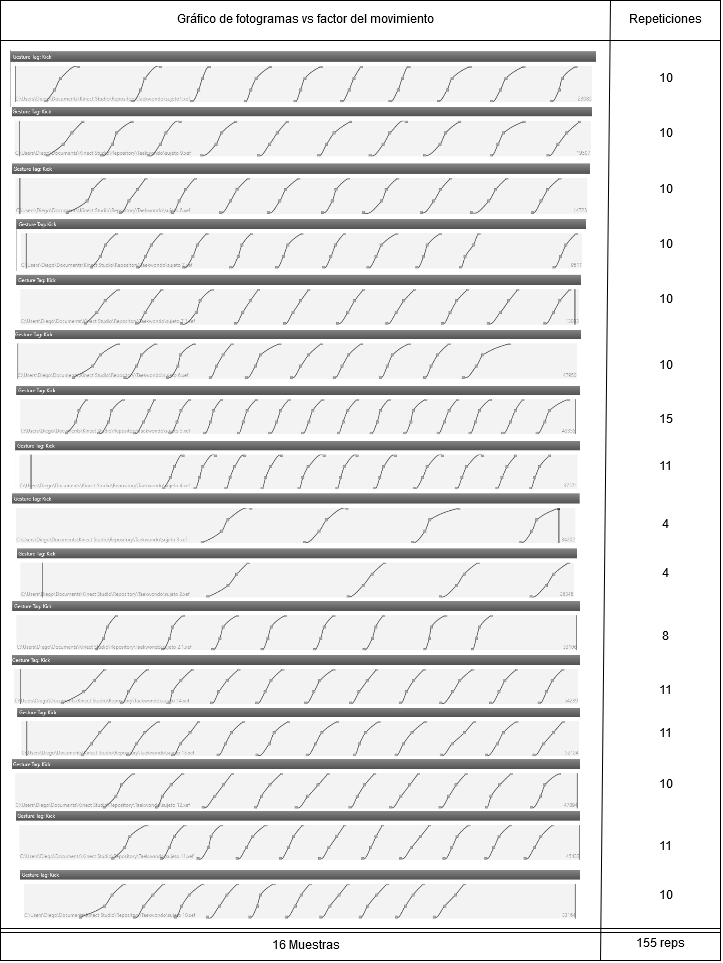
\includegraphics[width=445px,height=350px]{graphics/resultados/GraSegTaekwondo.PNG} \\
	\textbf{Fuente:} Recuperado por los v\'ideos etiquetados del trabajo de campo (ver instrumento \ref{ins:VisualGestureBuilder})
\end{table}
\section{Selecci\'on y pruebas del modelo} \label{res:chooseModel}
Por cada equipo deportivo se realiz\'o una tabla de informaci\'on del modelo de reconocimiento de los pasos de un movimiento v\'alido, la cual se divide en tres partes:
\begin{itemize}
\item  La primera parte se encontr\'o los errores del factor del movimiento de cada modelo y posteriormente se calcul\'o la media de cada error, la cual representa una \'idea de los  errores de todas las muestras de un equipo deportivo.
\item  La segunda parte se compone en la selecci\'on del submodelo que tenga la menor RECM (prioridad) y la menor DMA (se verifica en caso que exista dos o m\'as submodelos que tenga el mismo valor RECM), adem\'as de la aprobaci\'on o el rechazo de cada modelo (chequeando si el promedio RECM es menor a un medio del valor de identificaci\'on, con el fin objetivo de evitar colisiones de intervalos de confianzas en los pasos intermedios),  adem\'as de encontrar el porcentaje de recognition.
\item Finalmente, la tercera parte se muestra en caso que se apruebe el modelo, la cual detalla los intervalos de confianza para reconocer los pasos requeridos  de un movimiento.
\end{itemize}
\begin{table}[H]
\begin{center}
\caption{Modelos y pruebas del equipo de Taekwondo}
\label{tab:chooseTaekwondo}
\begin{tabular}{cccc}
\hline
\multicolumn{4}{|c|}{1. Datos de los errores de los submodelo} \\ \hline
\multicolumn{1}{|c|}{\textbf{Submodelo}} & \multicolumn{1}{c|}{\textbf{EMP}} & \multicolumn{1}{c|}{\textbf{DMA}} & \multicolumn{1}{c|}{\textbf{RECM}} \\ \hline
\multicolumn{1}{|c|}{1} & \multicolumn{1}{c|}{-0,03543} & \multicolumn{1}{c|}{0,301911} & \multicolumn{1}{c|}{+/-0,374544} \\ \hline
\multicolumn{1}{|c|}{2} & \multicolumn{1}{c|}{0,050888} & \multicolumn{1}{c|}{0,297433} & \multicolumn{1}{c|}{+/-0,393153} \\ \hline
\multicolumn{1}{|c|}{3} & \multicolumn{1}{c|}{0,200827} & \multicolumn{1}{c|}{0,214594} & \multicolumn{1}{c|}{+/-0,191583} \\ \hline
\multicolumn{1}{|c|}{\textbf{Promedio}} & \multicolumn{1}{c|}{0,072095} & \multicolumn{1}{c|}{0,271313} & \multicolumn{1}{c|}{+/-0,319760} \\ \hline
\multicolumn{1}{l}{} & \multicolumn{1}{l}{} & \multicolumn{1}{l}{} & \multicolumn{1}{l}{} \\ \hline
\multicolumn{4}{|c|}{2. Detalle del modelo} \\ \hline
\multicolumn{3}{|c|}{\textbf{Mejor submodelo}} & \multicolumn{1}{c|}{3} \\ \hline
\multicolumn{3}{|c|}{\textbf{Aprueba o rechaza el modelo}} & \multicolumn{1}{c|}{\begin{tabular}[c]{@{}c@{}}Rechaza\\ 0,31976  \textgreater{}= 0.125\end{tabular}} \\ \hline
\multicolumn{3}{|c|}{\textbf{Recognition}} & \multicolumn{1}{c|}{-27.90\%} \\ \hline
\multicolumn{4}{l}{\textbf{Fuente:} C\'alculo de intervalos de confianza (ver f\'ormula \ref{frm:rangoConfiabilidad})}
\end{tabular}
\end{center}
\end{table}
\begin{table}[H]
\begin{center}
\caption{Modelos y pruebas del equipo de tenis de mesa }
\label{tab:chooseModelTenis}
\begin{tabular}{cccc}
\hline
\multicolumn{4}{|c|}{1. Datos de los errores de los submodelos} \\ \hline
\multicolumn{1}{|c|}{\textbf{Submodelo}} & \multicolumn{1}{c|}{\textbf{EMP}} & \multicolumn{1}{c|}{\textbf{DMA}} & \multicolumn{1}{c|}{\textbf{RECM}} \\ \hline
\multicolumn{1}{|c|}{1} & \multicolumn{1}{c|}{0,175144} & \multicolumn{1}{c|}{0,217553} & \multicolumn{1}{c|}{+/-0,236069} \\ \hline
\multicolumn{1}{|c|}{2} & \multicolumn{1}{c|}{0,022738} & \multicolumn{1}{c|}{0,113367} & \multicolumn{1}{c|}{+/-0,140393} \\ \hline
\multicolumn{1}{|c|}{3} & \multicolumn{1}{c|}{0,139513} & \multicolumn{1}{c|}{0,260699} & \multicolumn{1}{c|}{+/-0,342375} \\ \hline
\multicolumn{1}{|c|}{\textbf{Promedio}} & \multicolumn{1}{c|}{0,112465} & \multicolumn{1}{c|}{0,197206} & \multicolumn{1}{c|}{+/-0,239612} \\ \hline
\multicolumn{1}{l}{} & \multicolumn{1}{l}{} & \multicolumn{1}{l}{} & \multicolumn{1}{l}{} \\ \hline
\multicolumn{4}{|c|}{2. Detalle del modelo} \\ \hline
\multicolumn{3}{|c|}{\textbf{Mejor submodelo}} & \multicolumn{1}{c|}{2} \\ \hline
\multicolumn{3}{|c|}{\textbf{Aprueba o rechaza el modelo}} & \multicolumn{1}{c|}{\begin{tabular}[c]{@{}c@{}}Aprueba\\ 0,239612 \textless 0.25\end{tabular}} \\ \hline
\multicolumn{3}{|c|}{\textbf{Recognition}} & \multicolumn{1}{c|}{52.08\%} \\ \hline
\multicolumn{1}{l}{} & \multicolumn{1}{l}{} & \multicolumn{1}{l}{} & \multicolumn{1}{l}{} \\ \hline
\multicolumn{4}{|c|}{3. Detalle del paso del movimiento} \\ \hline
\multicolumn{2}{|c|}{\textbf{Detallle}} & \multicolumn{2}{c|}{\textbf{Intervalo de confianza}} \\ \hline
\multicolumn{1}{|c|}{Paso} & \multicolumn{1}{c|}{Etiqueta} & \multicolumn{1}{c|}{Inferior} & \multicolumn{1}{c|}{Superior} \\ \hline
\multicolumn{1}{|c|}{1} & \multicolumn{1}{c|}{0} & \multicolumn{1}{c|}{0} & \multicolumn{1}{c|}{0,239612} \\ \hline
\multicolumn{1}{|c|}{2} & \multicolumn{1}{c|}{1} & \multicolumn{1}{c|}{0,760388} & \multicolumn{1}{c|}{1} \\ \hline
\multicolumn{4}{l}{\textbf{Fuente:} C\'alculo de intervalos de confianza (ver f\'ormula \ref{frm:rangoConfiabilidad})}
\end{tabular}
\end{center}
\end{table}
\begin{table}[H]
\begin{center}
\caption{Modelos y pruebas del equipo de animaci\'on}
\label{tab:chooseCheerleader}
\begin{tabular}{cccc}
\hline
\multicolumn{4}{|c|}{1. Datos de los errores de los submodelos} \\ \hline
\multicolumn{1}{|c|}{\textbf{Submodelo}} & \multicolumn{1}{c|}{\textbf{EMP}} & \multicolumn{1}{c|}{\textbf{DMA}} & \multicolumn{1}{c|}{\textbf{RECM}} \\ \hline
\multicolumn{1}{|c|}{1} & \multicolumn{1}{c|}{0,02323} & \multicolumn{1}{c|}{0,038519} & \multicolumn{1}{c|}{+/-0,046957} \\ \hline
\multicolumn{1}{|c|}{2} & \multicolumn{1}{c|}{0,080008} & \multicolumn{1}{c|}{0,083864} & \multicolumn{1}{c|}{+/-0,076391} \\ \hline
\multicolumn{1}{|c|}{3} & \multicolumn{1}{c|}{0,032244} & \multicolumn{1}{c|}{0,04105} & \multicolumn{1}{c|}{+/-0,045347} \\ \hline
\multicolumn{1}{|c|}{\textbf{Promedio}} & \multicolumn{1}{c|}{0,045161} & \multicolumn{1}{c|}{0,054478} & \multicolumn{1}{c|}{+/-0,056232} \\ \hline
\multicolumn{1}{l}{} & \multicolumn{1}{l}{} & \multicolumn{1}{l}{} & \multicolumn{1}{l}{} \\ \hline
\multicolumn{4}{|c|}{2. Detalle del modelo} \\ \hline
\multicolumn{3}{|c|}{\textbf{Mejor submodelo}} & \multicolumn{1}{c|}{3} \\ \hline
\multicolumn{3}{|c|}{\textbf{Aprueba o rechaza el modelo}} & \multicolumn{1}{c|}{\begin{tabular}[c]{@{}c@{}}Aprueba\\ 0,056232 \textless 0.165\end{tabular}} \\ \hline
\multicolumn{3}{|c|}{\textbf{Recognition}} & \multicolumn{1}{c|}{82.96\%} \\ \hline
\multicolumn{1}{l}{} & \multicolumn{1}{l}{} & \multicolumn{1}{l}{} & \multicolumn{1}{l}{} \\ \hline
\multicolumn{4}{|c|}{3. Detalle del paso del movimiento} \\ \hline
\multicolumn{2}{|c|}{\textbf{Detallle}} & \multicolumn{2}{c|}{\textbf{Intervalo de confianza}} \\ \hline
\multicolumn{1}{|c|}{Paso} & \multicolumn{1}{c|}{Etiqueta} & \multicolumn{1}{c|}{Inferior} & \multicolumn{1}{c|}{Superior} \\ \hline
\multicolumn{1}{|c|}{1} & \multicolumn{1}{c|}{0} & \multicolumn{1}{c|}{0} & \multicolumn{1}{c|}{0,056232} \\ \hline
\multicolumn{1}{|c|}{2} & \multicolumn{1}{c|}{0.5} & \multicolumn{1}{c|}{0,443768} & \multicolumn{1}{c|}{0,556232} \\ \hline
\multicolumn{1}{|c|}{3} & \multicolumn{1}{c|}{1} & \multicolumn{1}{c|}{0,943768} & \multicolumn{1}{c|}{1} \\ \hline
\multicolumn{4}{l}{\textbf{Fuente:} C\'alculo de intervalos de confianza (ver f\'ormula \ref{frm:rangoConfiabilidad})}
\end{tabular}
\end{center}
\end{table}
\section{Clasificaciones de movimiento v\'alidos e inv\'alidos} \label{res:clasiMov}
Estos resultados demuestran lo siguiente:
\begin{itemize}
\item  Cada submodelo fue entrenado con distintos datos de entrenamientos y testeos (adem\'as de mostrar los porcentajes de datos de entrenamientos y testeos).
\item Por cada v\'ideo de entrenamiento de cada submodelo, se determin\'o  las repeticiones v\'alidas e inv\'alidas (de acuerdo a los intervalos de confianza  y el algoritmo clasificador de repetici\'on de un movimiento v\'alido), as\'i mismo se observa que el mejor submodelo (submodelo que tiene la menor RECM y DMA) es el que tiene una mayor cantidad de volumen de repeticiones v\'alidas y una menor cantidad de volumen de repeticiones inv\'alidas.
\item A partir de las repeticiones inv\'alidas se pueden calcular el n\'umero de repeticiones inv\'alidas por no detectar el paso correspondiente (Es un par\'ametro que le puede ayudar al usuario a saber en cu\'al paso ha fallado los atletas de testeos). 
\end{itemize}
\begin{table}[H]
\begin{center}
\caption{C\'alculo de movimientos v\'alidos e inv\'alidos del equipo de animaci\'on}
\label{tab:validAnimacion}
\begin{tabular}{|c|c|c|c|c|c|c|c|}
\hline
\textbf{Detalles}    & \multicolumn{2}{c|}{\textbf{\begin{tabular}[c]{@{}c@{}}Las 1229 repeticiones\\  del movimiento\end{tabular}}}                          & \multicolumn{2}{c|}{\textbf{\begin{tabular}[c]{@{}c@{}}Las repeticiones \\ de testeos\end{tabular}}}                                      & \multicolumn{3}{c|}{\textbf{\begin{tabular}[c]{@{}c@{}}Las repeticiones son \\ inv\'alidas porque no se \\ detect\'o el paso No.\end{tabular}}} \\ \hline
\textbf{Submodelos}  & \textbf{\begin{tabular}[c]{@{}c@{}}De \\ entrenamientos\end{tabular}} & \textbf{\begin{tabular}[c]{@{}c@{}}De \\ testeos\end{tabular}} & \textbf{\begin{tabular}[c]{@{}c@{}}Son\\ v\'alidas\end{tabular}} & \textbf{\begin{tabular}[c]{@{}c@{}}Son \\ inv\'alidas\end{tabular}} & \textbf{Uno}                                     & \textbf{Dos}                                     & \textbf{Tres}                                    \\ \hline
1                    & 1053                                                                  & 176                                                            & 97                                                                & 79                                                                    & 2                                              & 25                                             & 52                                             \\ \hline
2                    & 1058                                                                  & 171                                                            & 50                                                                & 121                                                                   & 0                                              & 8                                              & 113                                            \\ \hline
3                    & 1055                                                                  & 174                                                            & 115                                                               & 59                                                                    & 0                                              & 43                                             & 16                                           \\ \hline
\textbf{Promedio}    & 1055                                                                  & 174                                                            & 88                                                                & 86                                                                    & 0                                              & 25                                             & 61                                            \\ \hline
\textbf{Porcentajes} & 85,84\%                                                               & 14,16\%                                                        & 50,57\%                                                           & 49,43\%                                                               & 0,00\%                                         & 29,07\%                                        & 70.93\%                                            \\ \hline
\multicolumn{8}{l}{\textbf{Fuente:} C\'alculo de porcentajes v\'alidos e inv\'alidos (ver F\'ormula \ref{frm:porcentajeClasificador})}
\end{tabular}
\end{center}
\end{table}

\begin{table}[H]
\begin{center}
\caption{C\'alculo de movimientos v\'alidos e inv\'alidos del equipo de tenis de mesa}
\label{tab:validTenis}
\begin{tabular}{|c|c|c|c|c|c|c|}
\hline
\textbf{Detalles}    & \multicolumn{2}{c|}{\textbf{\begin{tabular}[c]{@{}c@{}}Las 332 repeticiones\\  del movimiento\end{tabular}}}                           & \multicolumn{2}{c|}{\textbf{\begin{tabular}[c]{@{}c@{}}Las repeticiones \\ de testeos\end{tabular}}} & \multicolumn{2}{c|}{\textbf{\begin{tabular}[c]{@{}c@{}}Las repeticiones son \\ inv\'alidas porque no se \\ detect\'o el paso No.\end{tabular}}} \\ \hline
\textbf{Submodelos}  & \textbf{\begin{tabular}[c]{@{}c@{}}De \\ entrenamientos\end{tabular}} & \textbf{\begin{tabular}[c]{@{}c@{}}De \\ testeos\end{tabular}} & \textbf{Son v\'alidas}                                 & \textbf{Son inv\'alidas}                                & \textbf{Uno}                                                             & \textbf{Dos}                                                             \\ \hline
1                    & 282                                                                   & 50                                                             & 15                                               & 35                                                & 3                                                                      & 32                                                                     \\ \hline
2                    & 289                                                                   & 43                                                             & 38                                               & 5                                                 & 4                                                                      & 1                                                                      \\ \hline
3                    & 280                                                                   & 52                                                             & 41                                               & 11                                                & 2                                                                      & 9                                                                      \\ \hline
\textbf{Promedio}    & 283                                                                   & 49                                                             & 32                                               & 17                                                & 3                                                                      & 14                                                                     \\ \hline
\textbf{Porcentajes} & 85,24\%                                                               & 14,76\%                                                        & 65,31\%                                          & 34,69\%                                           & 17,65\%                                                                & 82,35\%                                                                \\ \hline
\multicolumn{7}{l}{\textbf{Fuente:} C\'alculo de porcentajes v\'alidos e inv\'alidos (ver F\'ormula \ref{frm:porcentajeClasificador})}
\end{tabular}
\end{center}
\end{table}
De igual manera, se an\'aliza si el modelo de clasificaci\'on es aceptable, bas\'andose en los porcentajes de referencias v\'alidas e inv\'alidas (determinados a partir de las posibles combinaciones de una repetici\'on inv\'alida y una repetici\'on v\'alida), lo cual se busca mejorar el porcentaje de referencia v\'alidas y por  consiguiente disminuir el porcentaje de referencia inv\'alidas:
\begin{table}[H]
\begin{center}
\caption{Aceptaci\'on del modelo de clasificaci\'on del equipo de animaci\'on}
\label{tab:acModAni}
\begin{tabular}{|l|l|l|l|}
\hline
\textbf{Descripci\'on} & \textbf{\% de referencia} & \textbf{\% real} & \textbf{Aceptable/Rechazado} \\ \hline
Repeticiones v\'alidas              & 25,00\%                   & 50,57\%          & Aceptable                    \\ \hline
Repeticiones inv\'alidas            & 75,00\%                   & 49,43\%          & Aceptable                    \\ \hline
\multicolumn{3}{|r|}{\textbf{El modelo es}}                         & Aceptable                    \\ \hline 
\multicolumn{4}{l}{\textbf{Fuente:} C\'alculo de porcentajes de referencias de v\'alidos e inv\'alidos (ver figura  \ref{fig:porcValido})}
\end{tabular}
\end{center}
\end{table}
\begin{table}[H]
\begin{center}
\caption{Aceptaci\'on del modelo de clasificaci\'on del equipo de tenis de mesa}
\label{tab:acModTenis}
\begin{tabular}{|l|l|l|l|}
\hline
\textbf{Descripci\'on} & \textbf{\% de referencia} & \textbf{\% real} & \textbf{Aceptable/Rechazado} \\ \hline
Repeticiones v\'alidas              & 33,00\%                   & 65,31\%          & Aceptable                    \\ \hline
Repeticiones inv\'alidas            & 67,00\%                   & 34,69\%          & Aceptable                    \\ \hline
\multicolumn{3}{|r|}{\textbf{El modelo es}}                         & Aceptable                    \\ \hline 
\multicolumn{4}{l}{\textbf{Fuente:} C\'alculo de porcentajes de referencias de v\'alidos e inv\'alidos (ver figura  \ref{fig:porcValido})}
\end{tabular}
\end{center}
\end{table}
\section{Interpretaci\'on de recognition} \label{res:recognition}
Estos resultados demuestran que al tener un valor recognition cercano al 100\%, reconocer\'a fotogramas similares a los fotogramas etiquetados de cada paso (lo esperado):
\begin{itemize}
\item  Para el equipo de animaci\'on, se identific\'o los fotogramas relacionados al paso dos, donde el valor esperado es cuando el factor de movimiento tiene un valor de 0.5 (etiqueta del paso dos). Sin embargo, se observa que el modelo reconoce un 82.96\% de los fotogramas parecidos a lo esperado (fotogramas que se encuentran dentro del intervalo de confianza del reconocimiento del paso dos), cuyas diferencias son unos peque\~nos desplazamientos en la parte inferior del cuerpo y brazos, mientras que los fotogramas debajo del valor de recognition, las diferencias de desplazamientos son m\'as notables (ya no son tan similares).
\item  Para el equipo de tenis de mesa, se aplic\'o  los fotogramas relacionados al paso uno, donde el valor esperado es cuando el factor de movimiento tiene un valor de 0 (etiqueta del paso uno). Sin embargo, se observa que el modelo reconoce un 52.08\% de los fotogramas parecidos a lo esperado (fotogramas que se encuentran dentro del intervalo de confianza del reconocimiento del paso uno), esto conlleva a reconocer aquellos fotogramas donde el saque no ha llegado a la distancia frontal (cara), mientras que los fotogramas por abajo del valor de recognition, son aquellos que han cruzado la distancia frontal.
\end{itemize}
\begin{table}[H]
	\caption{Interpretaci\'on del valor de recognition del paso dos de un jumping jack}
	\label{fig:recognitionJumpingJack}
	\centering
	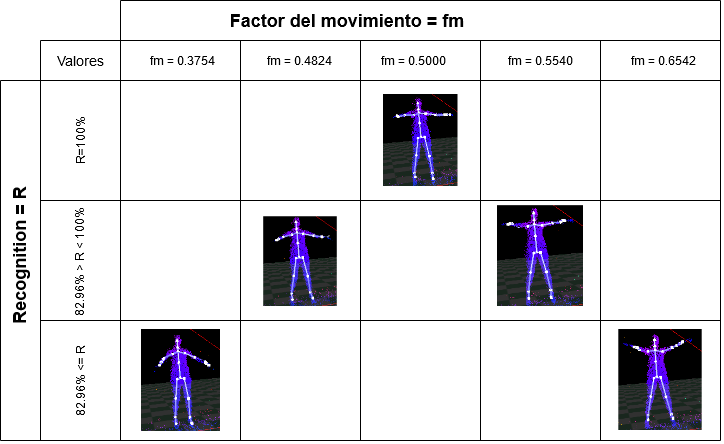
\includegraphics[width=445px,height=220px]{graphics/resultados/recognitionChe.PNG} \\
	\textbf{Fuente:} Recuperado por los v\'ideos etiquetados del trabajo de campo (ver instrumento \ref{ins:VisualGestureBuilder}).
\end{table}
\begin{table}[H]
	\caption{Interpretaci\'on del valor de recognition del paso uno de un saque derecha}
	\label{fig:recognitionSaque}
	\centering
	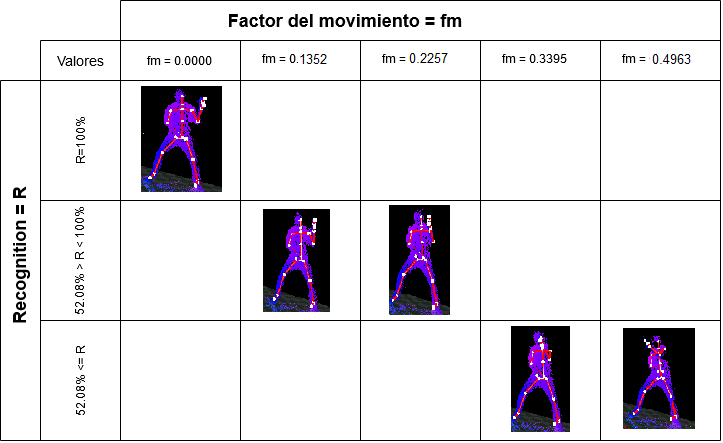
\includegraphics[width=445px,height=220px]{graphics/resultados/RecognitionTen.PNG} \\
	\textbf{Fuente:} Recuperado por los v\'ideos etiquetados del trabajo de campo (ver instrumento \ref{ins:VisualGestureBuilder}).
\end{table}
\section{El modelo reconoce solo el movimiento analizado} \label{res:recoMovAna}
Estos resultados demuestran que el factor del movimiento de cada movimiento analizado busca reconocer todos los pasos del movimiento analizado (debido que los factores del movimiento se encuentran en todos los intervalos de confianza de cada equipo deportivo), la cual se realiz\'o un cuadro comparativo entre jumping jack y un saque derecha, donde se comparan los factores de los movimientos:
\begin{itemize}
\item  Durante la ejecuci\'on de un saque derecha, el factor del movimiento de saque derecha reconoce el paso uno y dos (debido que los factores de movimiento se encuentran en sus respectivos intervalos de confianza del equipo de  tenis de mesa). Mientras que el factor del movimiento de jumping jack reconoce el paso uno durante esos dos fotogramas (debido que los factores de movimiento se encuentran en el intervalo de confianza del paso uno del equipo de tenis de mesa).
\item  Durante la ejecuci\'on de un jumping jack, el factor del movimiento de jumping jack reconoce el paso uno, dos y tres (debido que los factores de movimiento se encuentran en sus respectivos intervalos de confianza del equipo de animaci\'on), mientras que el factor del movimiento de saque derecha no est\'a reconociendo ning\'un paso (debido que los factores de movimiento no se encuentran en ning\'un intervalo de confianza del equipo de animaci\'on).
\end{itemize}
\begin{table}[H]
	\caption{Cuadro comparativo entre un jumping jack y saque derecha}
	\label{fig:comparativeMovements}
	\centering
	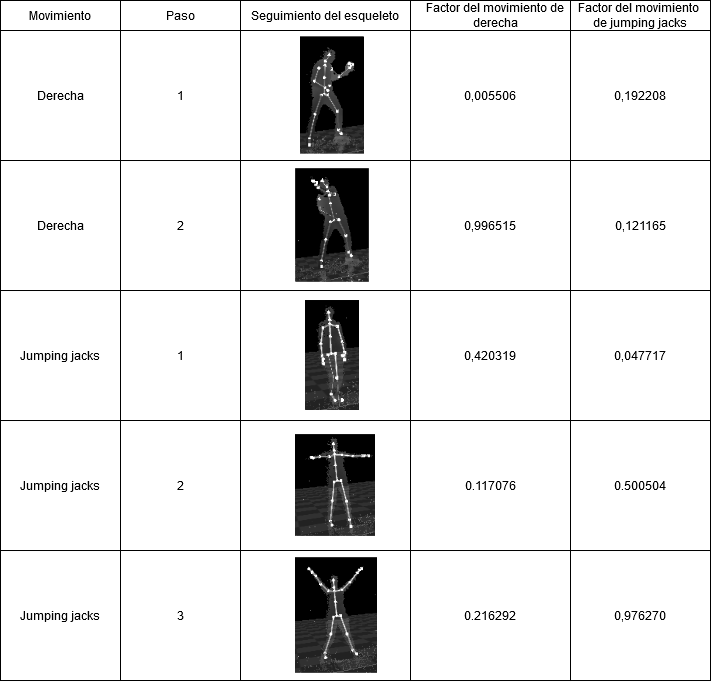
\includegraphics[width=445px,height=440px]{graphics/resultados/compFM.PNG} \\
	\textbf{Fuente:} Recuperado por los v\'ideos etiquetados del trabajo de campo (ver instrumento \ref{ins:VisualGestureBuilder}).
\end{table}
\section{Muestras de regresiones de los movimientos} \label{res:regretions}
Estos resultados muestran:
\begin{itemize}
\item  Un ejemplo de las posibles regresiones (para este caso se analiz\'o una l\'inea de tendencia de grado 3) que pueden implementar cada \'arbol de regresi\'on del algoritmo Random Forest Regression.
\item  Comprobar que los modelos aceptados fueron entrenados con distintos datos de entrenamientos (uniformidad con los tiempos de capturas y una dispersi\'on con los recorridos de una articulaci\'on, durante la ejecuci\'on del  movimiento).
\item  El tiempo m\'aximo de una repetici\'on de un movimiento v\'alido o inv\'alido (el peor de los casos para ejecutar una repetici\'on), esto quiere  decir que para ejecutar un jumping jack se requiere a lo m\'aximo 0.53 segundos, mientras que para un saque derecha se requiere a lo m\'aximo 0.73 segundos.
\end{itemize}

\begin{figure}[H]
	\caption{Regresi\'on distancia versus tiempo, del equipo animaci\'on}
	\label{fig:regrCheerleader}
	\centering
	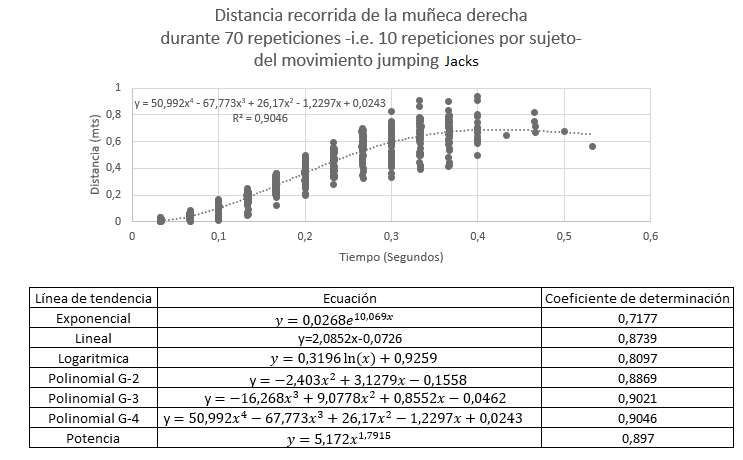
\includegraphics[width=445px,height=180px]{graphics/resultados/cluster-cheerleaders.PNG} \\
	\textbf{Fuente:} Recuperado por los v\'ideos etiquetados del trabajo de campo.
\end{figure}
\begin{figure}[H]
	\caption{Regresi\'on distancia versus tiempo  del equipo de tenis de mesa}
	\label{fig:regrTennisDeMesa}
	\centering
	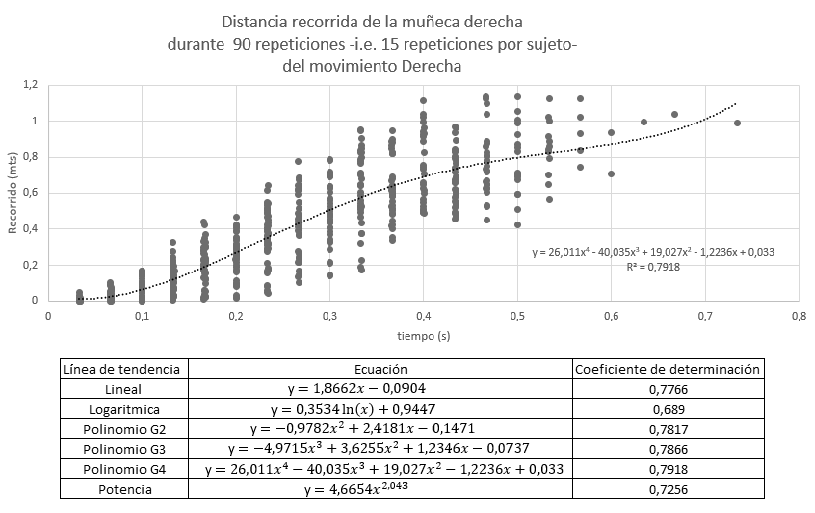
\includegraphics[width=445px,height=180px]{graphics/resultados/cluster-tennis.PNG} \\
	\textbf{Fuente:} Recuperado por los v\'ideos etiquetados del trabajo de campo.
\end{figure}
\section{Reconocimiento de movimiento}
En esta secci\'on se ense\~na los resultados de la interfaz gr\'afica del reconocimiento de repeticiones de un movimiento, la cual est\'a conformado por un conjunto de im\'agenes que muestran el seguimiento del esqueleto durante la ejecuci\'on de una repetici\'on, as\'i mismo en cada imagen se muestra los siguientes detalles:
\begin{itemize}
\item \textbf{Estado:} Tiene el valor de trabajo, debido que fue capturado durante el tiempo de trabajo en una rutina de tabata.
\item \textbf{Temporizador:} Tiempo de cuenta regresiva, la cual indica cu\'antos segundos le quedan al atleta en el estado de trabajo.
\item \textbf{Serie:} Le indica al atleta, cu\'al n\'umero de serie se est\'a ejecutando (los resultados fueron capturado durante la serie No. 1 de trabajo).
\item \textbf{Repeticiones:} Le muestran al atleta la cantidad de repeticiones que lleva durante una   serie de trabajo (se debe observar que este indicador incrementa en el \'ultimo paso de cada movimiento).
\item \textbf{Paso:} N\'umero que indica el \'ultimo paso ejecutado (comenzando desde el valor 0). Se debe tomar en cuenta que dicho valor cambia dependiendo del factor de movimiento (progreso). Es decir, se  reconoce cada paso del movimiento, ya que el valor del progreso se encuentra dentro de alg\'un intervalo de confianza (Ver las tablas de resultados de selecci\'on y pruebas del modelo).
\item \textbf{Progreso:} Factor del movimiento en tiempo real (obtenido a partir del algoritmo Random Forest Regression), la cual va incrementado por cada paso que avance el atleta.
\item \textbf{Tiempo total:} Tiempo total que lleva actualmente el atleta. En los resultados se pueden ver que el atleta emplea una repetici\'on en per\'iodos de segundos, esto quiere decir que el atleta tard\'o 1.089 segundos durante el movimiento derecha y  0.363 segundos para un jumping jack.
\end{itemize}
\begin{figure}[H]
	\caption{Reconocimiento del movimiento derecha}
	\label{fig:recognitionTenis}
	\centering
	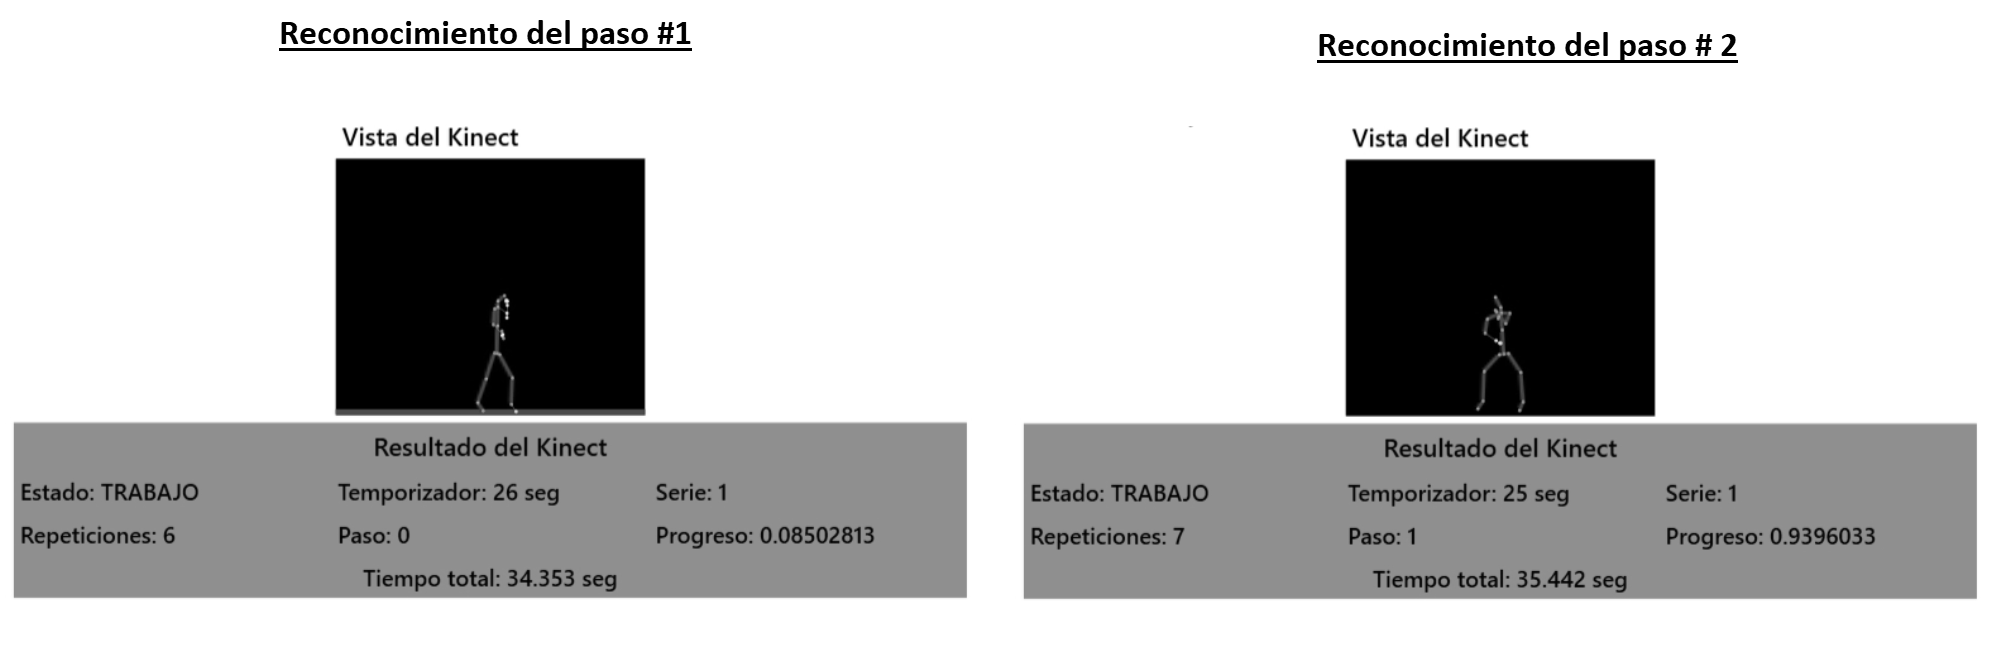
\includegraphics[width=420px,height=250px]{graphics/resultados/recognitionTennis.png} \\
	\textbf{Fuente:} Sujeto de validaci\'on del modelo en tiempo real.
\end{figure}
\begin{figure}[H]
	\caption{Reconocimiento del movimiento jumping jacks}
	\label{fig:recognitionCheerleader}
	\centering
	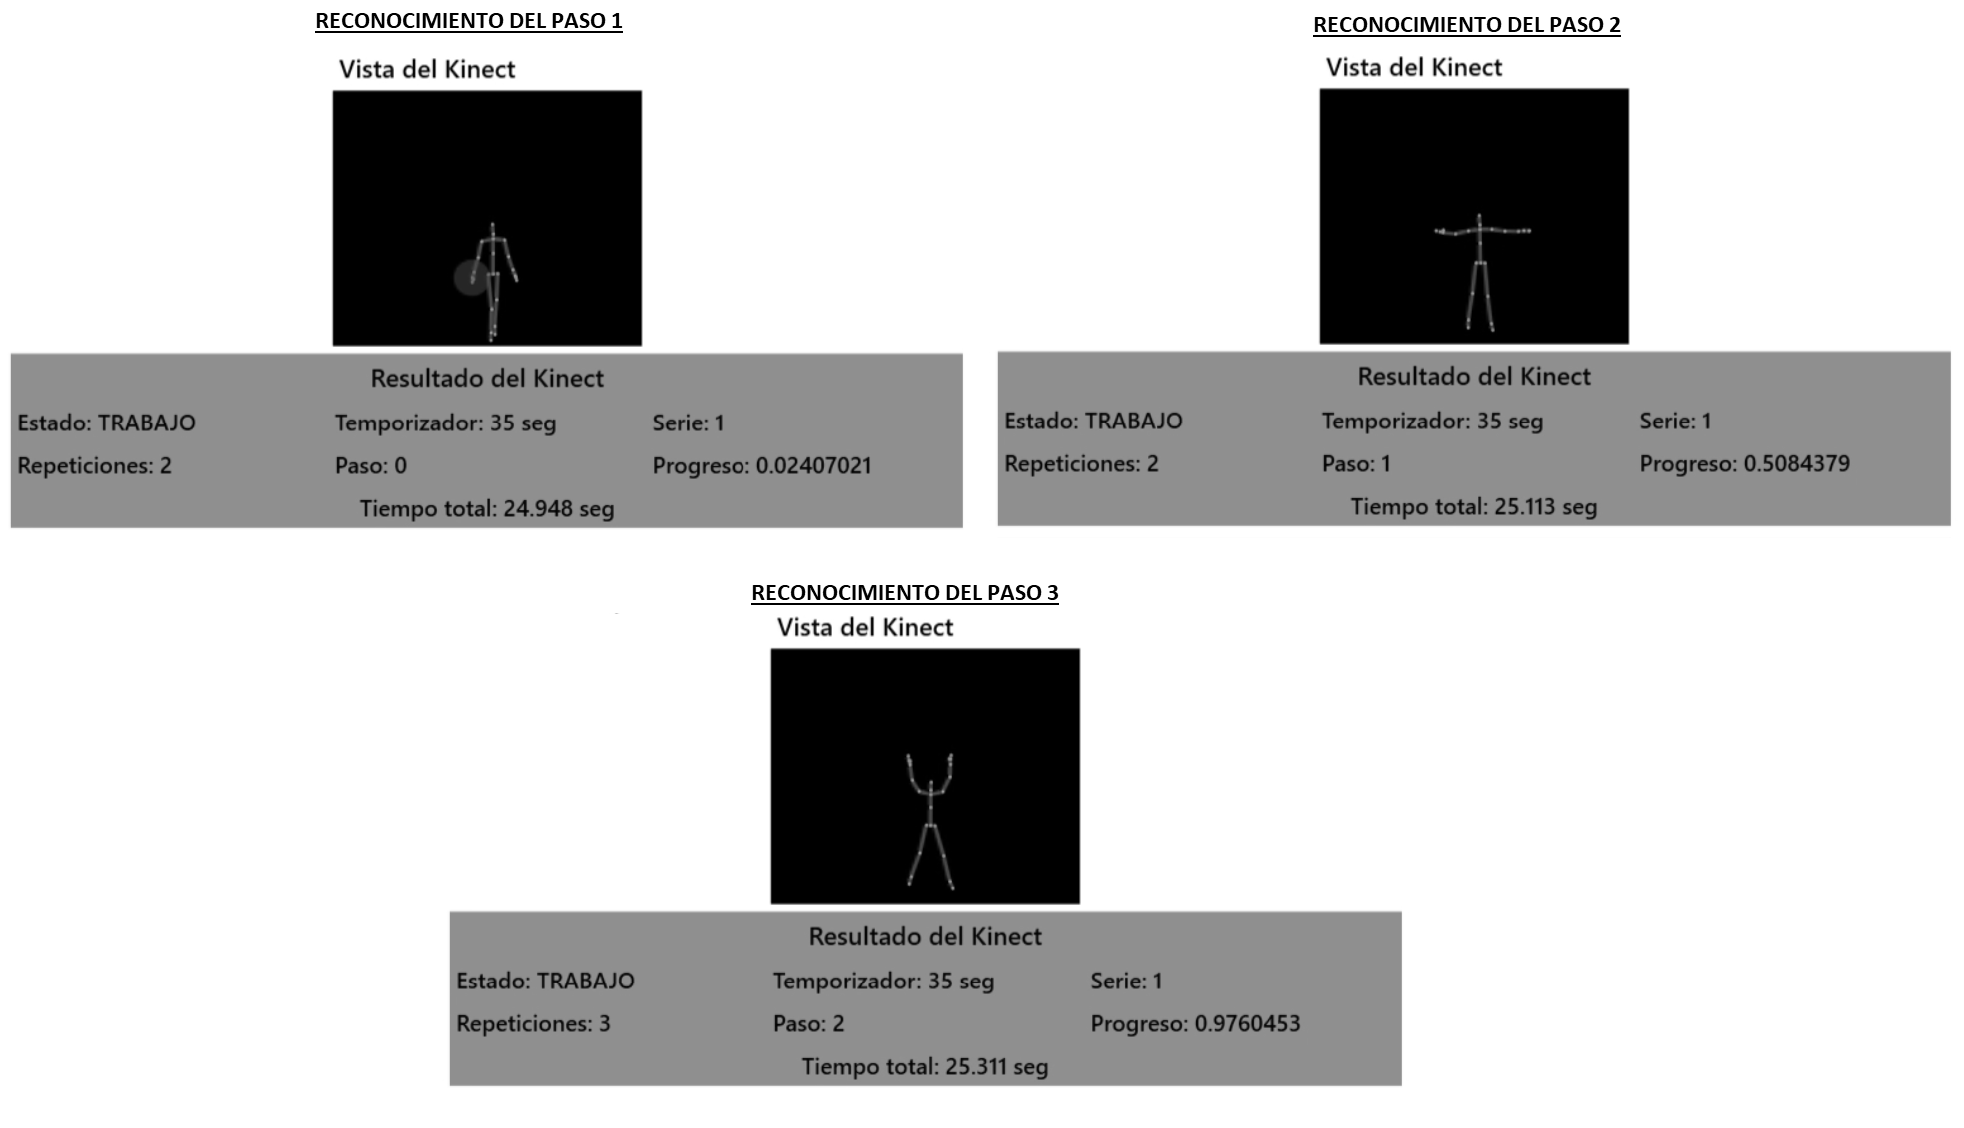
\includegraphics[width=430px,height=320px]{graphics/resultados/recognitionCheerleader.png} \\
	\textbf{Fuente:} Sujeto de validaci\'on del modelo en tiempo real.
\end{figure}
\section{Resultados de los sujetos de validaci\'on} \label{res:valResults}
A continuaci\'on se presenta la interfaz gr\'afica de los resultados de la rutina tabata por equipo deportivo, con las siguientes caracter\'isticas de los atletas:
\begin{itemize}
\item Se utilizaron atletas que no participaron en la toma de datos iniciales (entrenamientos y testeos del modelo).
\item Se utilizaron atletas que ten\'ian  condiciones adecuadas (vestuarios adecuados, buena alimentaci\'on,  buena salud f\'isica).
\item Se utilizaron atletas que realizar\'on su rutina de estiramiento y calentamiento previamente al entrenamiento (con el fin de objetivo de preparar el cuerpo humano).
\item Se utilizaron atletas que saben ejecutar repeticiones v\'alidas (conocen todos los pasos del movimiento). 
\end{itemize}
\medbreak
Por otro lado, estos resultados se dividen en dos partes:
\begin{itemize}
\item La primera parte consta de un conjunto de gr\'aficas que muestra de manera visual, los per\'iodos de trabajos (tiempos en donde estaban ejecutando repeticiones v\'alidas)
\item La segunda parte es un cuadro que detalla el  resumen ejecutivo de los resultados de la rutina tabata, en donde se muestran la velocidad de repeticiones de un movimiento v\'alido (medici\'on de unas de las habilidades f\'isicas de un atleta).
\end{itemize}
\begin{landscape}
\begin{chart}[H]
	\caption{Resultados del tabata del equipo de tenis de mesa}
	\label{fig:resTabTennis}
	\centering
	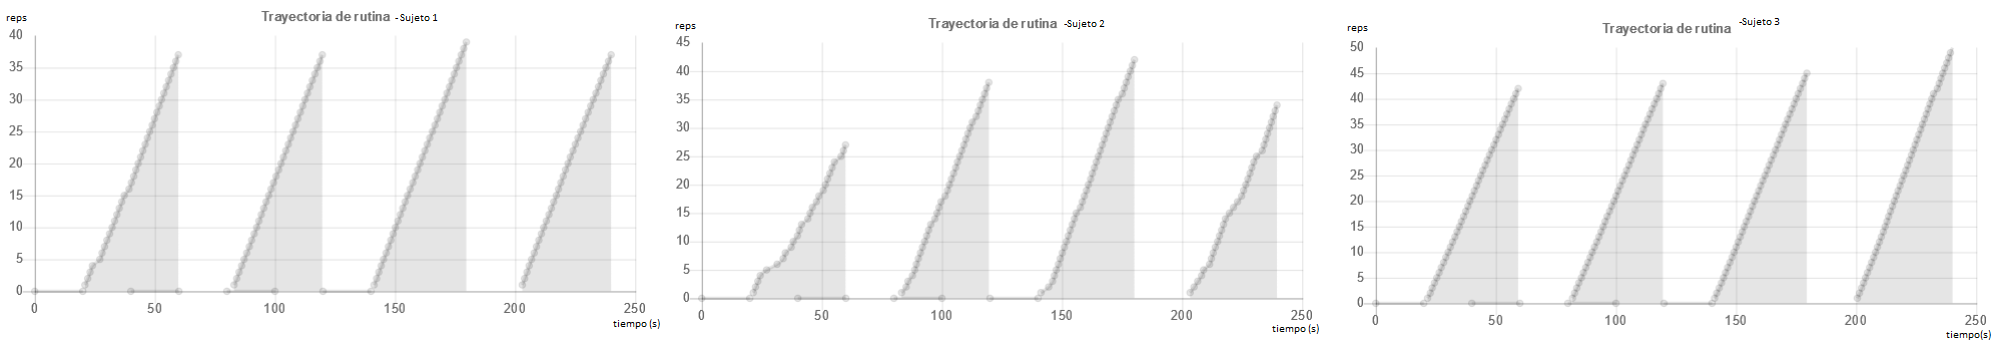
\includegraphics[width=610px,height=200px]{graphics/resultados/ResultRecognitionTenis.png} \\
	\textbf{Fuente:} Realizado con base a las observaciones del proceso de validaci\'on.
\end{chart}
\begin{table}[H]
\begin{center}
\caption{Detalle de la rutina tabata del equipo de tenis de mesa}
\label{tab:detailResultsTennis}
\begin{tabular}{|l|l|l|l|l|l|l|l|l|l|}
\hline
\textbf{Series} & \textbf{\begin{tabular}[c]{@{}l@{}}Trabajo\\ (segs)\end{tabular}} & \textbf{\begin{tabular}[c]{@{}l@{}}Descanso\\ (segs)\end{tabular}} & \textbf{\begin{tabular}[c]{@{}l@{}}Duraci\'on\\ (segs)\end{tabular}} & \textbf{Sujeto} & \textbf{\begin{tabular}[c]{@{}l@{}}Volumen de\\ repeticiones\end{tabular}} & \textbf{\begin{tabular}[c]{@{}l@{}}Repeticiones\\ m\'aximas en una\\ serie\end{tabular}} & \textbf{\begin{tabular}[c]{@{}l@{}}Tiempo m\'inimo\\ en una serie\\ (segs)\end{tabular}} & \textbf{\begin{tabular}[c]{@{}l@{}}Repeticiones \\ promedio por\\ serie\end{tabular}} & \textbf{\begin{tabular}[c]{@{}l@{}}Tiempo \\ promedio por\\ repetici\'on (segs)\end{tabular}} \\ \hline
\multirow{3}{*}{4} & \multirow{3}{*}{40} & \multirow{3}{*}{20} & \multirow{3}{*}{240} & 1 & 150 & 39 & 38.5440 & 38 & 0.7106 \\ \cline{5-10} 
 &  &  &  & 2 & 141 & 42 & 39.1050 & 35 & 0.7869 \\ \cline{5-10} 
 &  &  &  & 3 & 180 & 50 & 39.7980 & 45 & 0.3599 \\ \hline
 \multicolumn{10}{l}{\textbf{Fuente:} Gr\'afica de resultados del tabata del equipo de tenis de mesa}
\end{tabular}
\end{center}
\end{table}
\begin{chart}[H]
	\caption{Resultados del tabata del equipo de animaci\'on}
	\label{fig:resTabCheerleader}
	\centering
	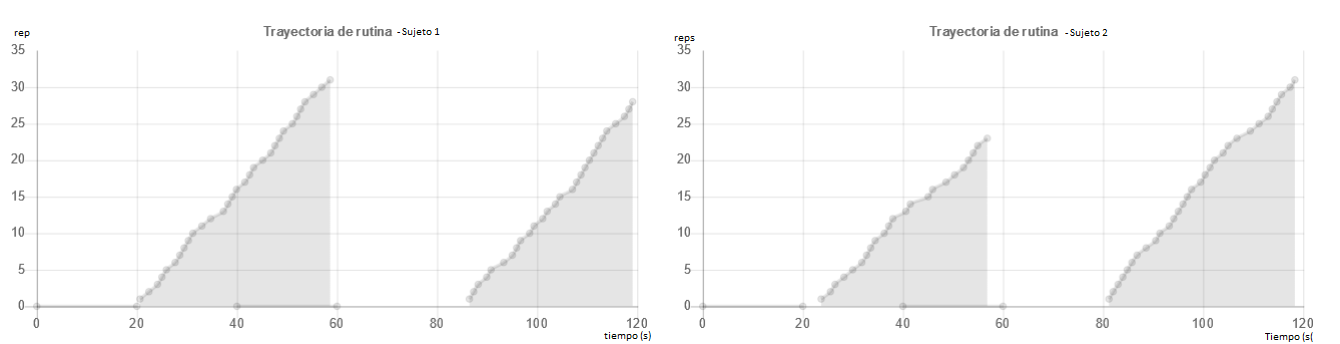
\includegraphics[width=610px,height=200px]{graphics/resultados/ResultRecognitionCheerleader.png} \\
	\textbf{Fuente:} Realizado con base a las observaciones del proceso de validaci\'on.
\end{chart}
\begin{table}[H]
\begin{center}
\caption{Detalle de la rutina tabata del equipo de animaci\'on}
\label{tab:detailResultsCheerleader}
\begin{tabular}{|l|l|l|l|l|l|l|l|l|l|}
\hline
\textbf{Series} & \textbf{\begin{tabular}[c]{@{}l@{}}Trabajo\\ (segs)\end{tabular}} & \textbf{\begin{tabular}[c]{@{}l@{}}Descanso\\ (segs)\end{tabular}} & \textbf{\begin{tabular}[c]{@{}l@{}}Duraci\'on\\ (segs)\end{tabular}} & \textbf{Sujeto} & \textbf{\begin{tabular}[c]{@{}l@{}}Volumen de\\ repeticiones\end{tabular}} & \textbf{\begin{tabular}[c]{@{}l@{}}Repeticiones\\ m\'aximas en una\\ serie\end{tabular}} & \textbf{\begin{tabular}[c]{@{}l@{}}Tiempo m\'inimo\\ en una serie\\ (segs)\end{tabular}} & \textbf{\begin{tabular}[c]{@{}l@{}}Repeticiones \\ promedio por\\ serie\end{tabular}} & \textbf{\begin{tabular}[c]{@{}l@{}}Tiempo \\ promedio por\\ repetici\'on (segs)\end{tabular}} \\ \hline
\multirow{2}{*}{2} & \multirow{2}{*}{40} & \multirow{2}{*}{20} & \multirow{2}{*}{120} & 1 & 59 & 31 & 38.3130 & 30 & 0.8284 \\ \cline{5-10} 
 &  &  &  & 2 & 54 & 31 & 37.5210 & 27 & 0.9301 \\ \hline
 \multicolumn{10}{l}{\textbf{Fuente} Gr\'afica de resultados del tabata del equipo de animaci\'on}
\end{tabular}
\end{center}
\end{table}
\end{landscape}
\section{Validaci\'on del modelo clasificador de los pasos requeridos de un movimiento v\'alido,  ejecutado por los sujetos de validaci\'on} \label{res:valResults}
Estos resultados demuestran si el modelo funciona de acuerdo al peor de los casos de una repetici\'on del movimiento v\'alido, tomando en cuenta los siguientes aspectos:
\begin{itemize}
\item Sujetos para la validaci\'on.
\item El tiempo de trabajo de la rutina tabata que fue programado a los sujetos de validaci\'on.
\item El tiempo m\'aximo para ejecutar una repetici\'on de un movimiento, realizados por los sujetos de pruebas y entrenamientos (ver secci\'on de muestras de regresiones de los movimientos).
\item El pron\'ostico de repeticiones totales de los sujetos de validaci\'on (de acuerdo al tiempo m\'aximo de una repetici\'on de lo sujetos de pruebas).
\item El porcentaje de repeticiones v\'alidas de cada movimiento deportivo (ver secci\'on de clasificaciones de movimientos v\'alidos e inv\'alidos).
\item El pron\'ostico de repeticiones v\'alidas de cada sujeto de validaci\'on (determinado a partir del porcentaje de repeticiones v\'alidas y el total de repeticiones pronosticadas).
\item Las repeticiones promedios por cada serie que realiz\'o el sujeto de validaci\'on durante su rutina de tabata (ver secci\'on de resultados de los sujetos de validaci\'ion).
\item  Ajuste del porcentaje de repetici\'on v\'alidas, la cual compara las repeticiones realizadas respecto a las pronosticadas.
\end{itemize}
De acuerdo a todos los aspectos, se observa que los  modelos clasificadores de los pasos requeridos de los movimientos v\'alidos de tenis de mesa y animaci\'on, detectaron m\'as repeticiones con respecto al peor de los casos de cada modelo deportivo (debido a que sus ajustes de porcentuales de repeticiones v\'alidas son positivos):
\begin{landscape}
\begin{table}[H]
\begin{center}
\caption{Validaci\'on de los resultados de tenis de mesa}
\label{tab:validationtenis}
\begin{tabular}{|c|c|c|c|c|c|c|c|}
\hline
\textbf{Sujetos} & \textbf{\begin{tabular}[c]{@{}c@{}}Tiempo de\\ trabajo (seg)\end{tabular}} & \textbf{\begin{tabular}[c]{@{}c@{}}Tiempo (seg) por\\ repetici\'on \\ pronosticada\end{tabular}} & \textbf{\begin{tabular}[c]{@{}c@{}}Repeticiones\\ pronosticadas\end{tabular}} & \textbf{\begin{tabular}[c]{@{}c@{}}Porcentaje de\\ repetici\'on \\ v\'alida\end{tabular}} & \textbf{\begin{tabular}[c]{@{}c@{}}Repeticiones\\ pronosticadas\\ v\'alidas\end{tabular}} & \textbf{\begin{tabular}[c]{@{}c@{}}Repeticiones\\ v\'alidas y \\ realizadas\end{tabular}} & \textbf{\begin{tabular}[c]{@{}c@{}}Ajuste del \\ porcentaje de \\ repetici\'on v\'alida\end{tabular}} \\ \hline
1                & 40                                                                   & 0,73                                                                                     & 54                                                                            & 65,31\%                                                                               & 35                                                                                      & 38                                                                                      & 8,57\%                                                                                            \\ \hline
2                & 40                                                                   & 0,73                                                                                     & 54                                                                            & 65,31\%                                                                               & 35                                                                                      & 35                                                                                      & 0,00\%                                                                                            \\ \hline
3                & 40                                                                   & 0,73                                                                                     & 54                                                                            & 65,31\%                                                                               & 35                                                                                      & 45                                                                                      & 28,57\%                                                                                           \\ \hline
\multicolumn{7}{|r|}{\textbf{Promedio}}                                                                                                                                                                                                                                                                                                                                                                                                                                                                                                        & 12,38\%                                                                                           \\ \hline
 \multicolumn{8}{l}{\textbf{Fuente:} Propia}
\end{tabular}
\end{center}
\end{table}

\begin{table}[H]
\begin{center}
\caption{Validaci\'on de los resultados de animaci\'on }
\label{tab:validationAnimation}
\begin{tabular}{|c|c|c|c|c|c|c|c|}
\hline
\textbf{Sujetos} & \textbf{\begin{tabular}[c]{@{}c@{}}Tiempo de\\ trabajo (seg)\end{tabular}} & \textbf{\begin{tabular}[c]{@{}c@{}}Tiempo por\\ repetici\'on \\ pronosticada (seg)\end{tabular}} & \textbf{\begin{tabular}[c]{@{}c@{}}Repeticiones\\ pronosticadas\end{tabular}} & \textbf{\begin{tabular}[c]{@{}c@{}}Porcentaje de\\ repetici\'on \\ v\'alida\end{tabular}} & \textbf{\begin{tabular}[c]{@{}c@{}}Repeticiones\\ pronosticadas\\ v\'alidas\end{tabular}} & \textbf{\begin{tabular}[c]{@{}c@{}}Repeticiones\\ v\'alidas y \\ realizadas\end{tabular}} & \textbf{\begin{tabular}[c]{@{}c@{}}Ajuste del \\ porcentaje de \\ repetici\'on v\'alida\end{tabular}} \\ \hline
1                & 40                                                                   & 0,53                                                                                     & 75                                                                            & 50,57\%                                                                               & 37                                                                                      & 59                                                                                      & 59,46\%                                                                                           \\ \hline
2                & 40                                                                   & 0,53                                                                                     & 75                                                                            & 50,57\%                                                                               & 37                                                                                      & 54                                                                                      & 45,95\%                                                                                           \\ \hline
\multicolumn{7}{|r|}{\textbf{Promedio}}                                                                                                                                                                                                                                                                                                                                                                                                                                                                                                        & 52,70\%                                                                                           \\ \hline
 \multicolumn{8}{l}{\textbf{Fuente:} Propia}
\end{tabular}
\end{center}
\end{table}
\end{landscape}